\section*{Introduction \& Background}

Often the case, researchers and scientists and interested in examining and making conclusions about the arrangement of molecules in certain substances. There are many methodologies of accomplishing this task but a simple one is a visual representation of the probabilities of atoms with respect to each other.
This particular measure is known as the \textbf{pairwise correlation function (also known as the radial distribution function)}. Given a particle at a position, this function calculates the probability of finding another particle at a distance of $r$ away from a given reference particle. Here is an example of what the output plot looks like:

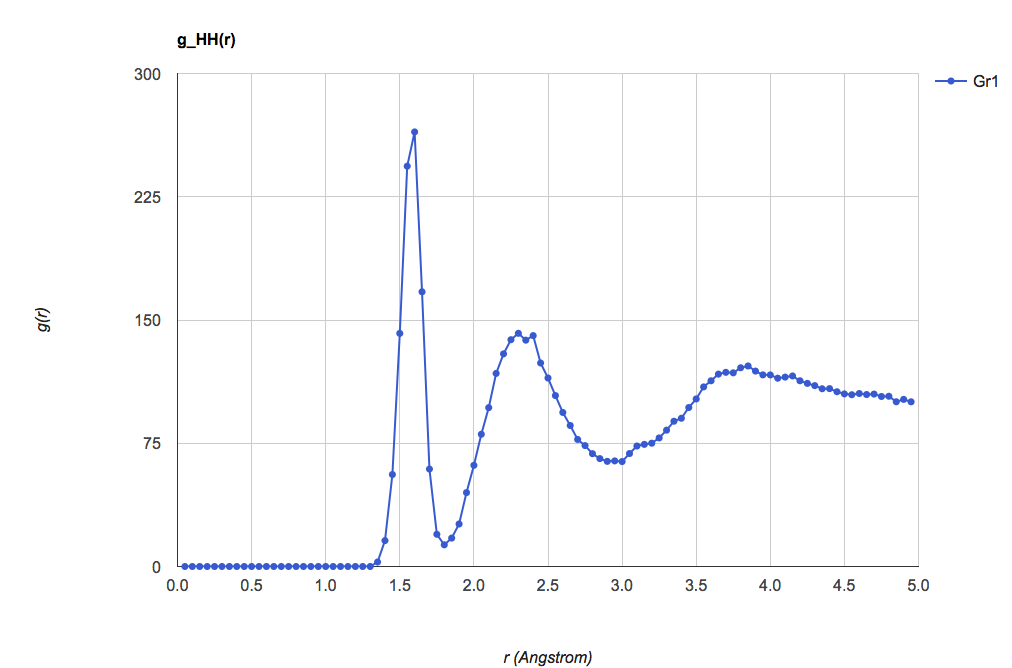
\includegraphics[width=0.90\textwidth]{sample_plot}

Interpreting the above plot is simple, yet very powerful and meaningful. The graph in the figure represents a water molecule. In particular, it quantitatively provides the probability of finding a hydrogen atom given a hydrogen atom. Looking at the graph, certain inferences can be made such as given a reference hydrogen atom, the probability of finding another hydrogen atom is virtually 0 until a radius of about 1.4, at the point which the probability of finding the particle increases. As larger radii are examined, the curve levels out which indicates that the probability of finding another hydrogen atom is averaged. 


In terms of the algorithm, the number of particles are measured between a radius \textit{r} and a delta radius, \textit{dr}. The correlation function is often calculated by finding the distances between all the particles and constructing the histogram based on the arrangement.

The resultant graph of the density of the molecules as a function of the radius is quite useful in understanding the molecular structure of substances as explained above. 

The general algorithm can be summarized as follows:

\begin{verbatim}
    1. Choose a value for dr and a radius value of r
    2. Count each particle that is at a distance of r and r + dr. 
    (This is essentially finding all the particles around the reference 
    particle arranged in a spherical shell).
    3. Divide the total count by N,  the total number of particles in 
    the given data.
    4. ???? . Not sure about the remaining steps.
    5. Then divide the number by 4 pi r^2 dr.    
\end{verbatim}

Another concept to mention here is the concept of \textit{folding}. When the molecular environment being considered is bounded, certain adjustments have to be made with respect to the distances of the atoms. In other words, if one atom is ``close to'' or ''on the boundaries'', an equivalent atom which is close to the reference atom has to be considered and the distance has to be \textit{folded or recalculated.} This is one of the main preprocessing step before performing the pairwise distance calculation around the reference particle (step 2). 

(Sorry, I do not know how to descriptively describe the concept of folding in simple words, so any help would be appreciated). 
